\begin{figure}[!htbp] \centering
\subsection{BDD Hardware}
{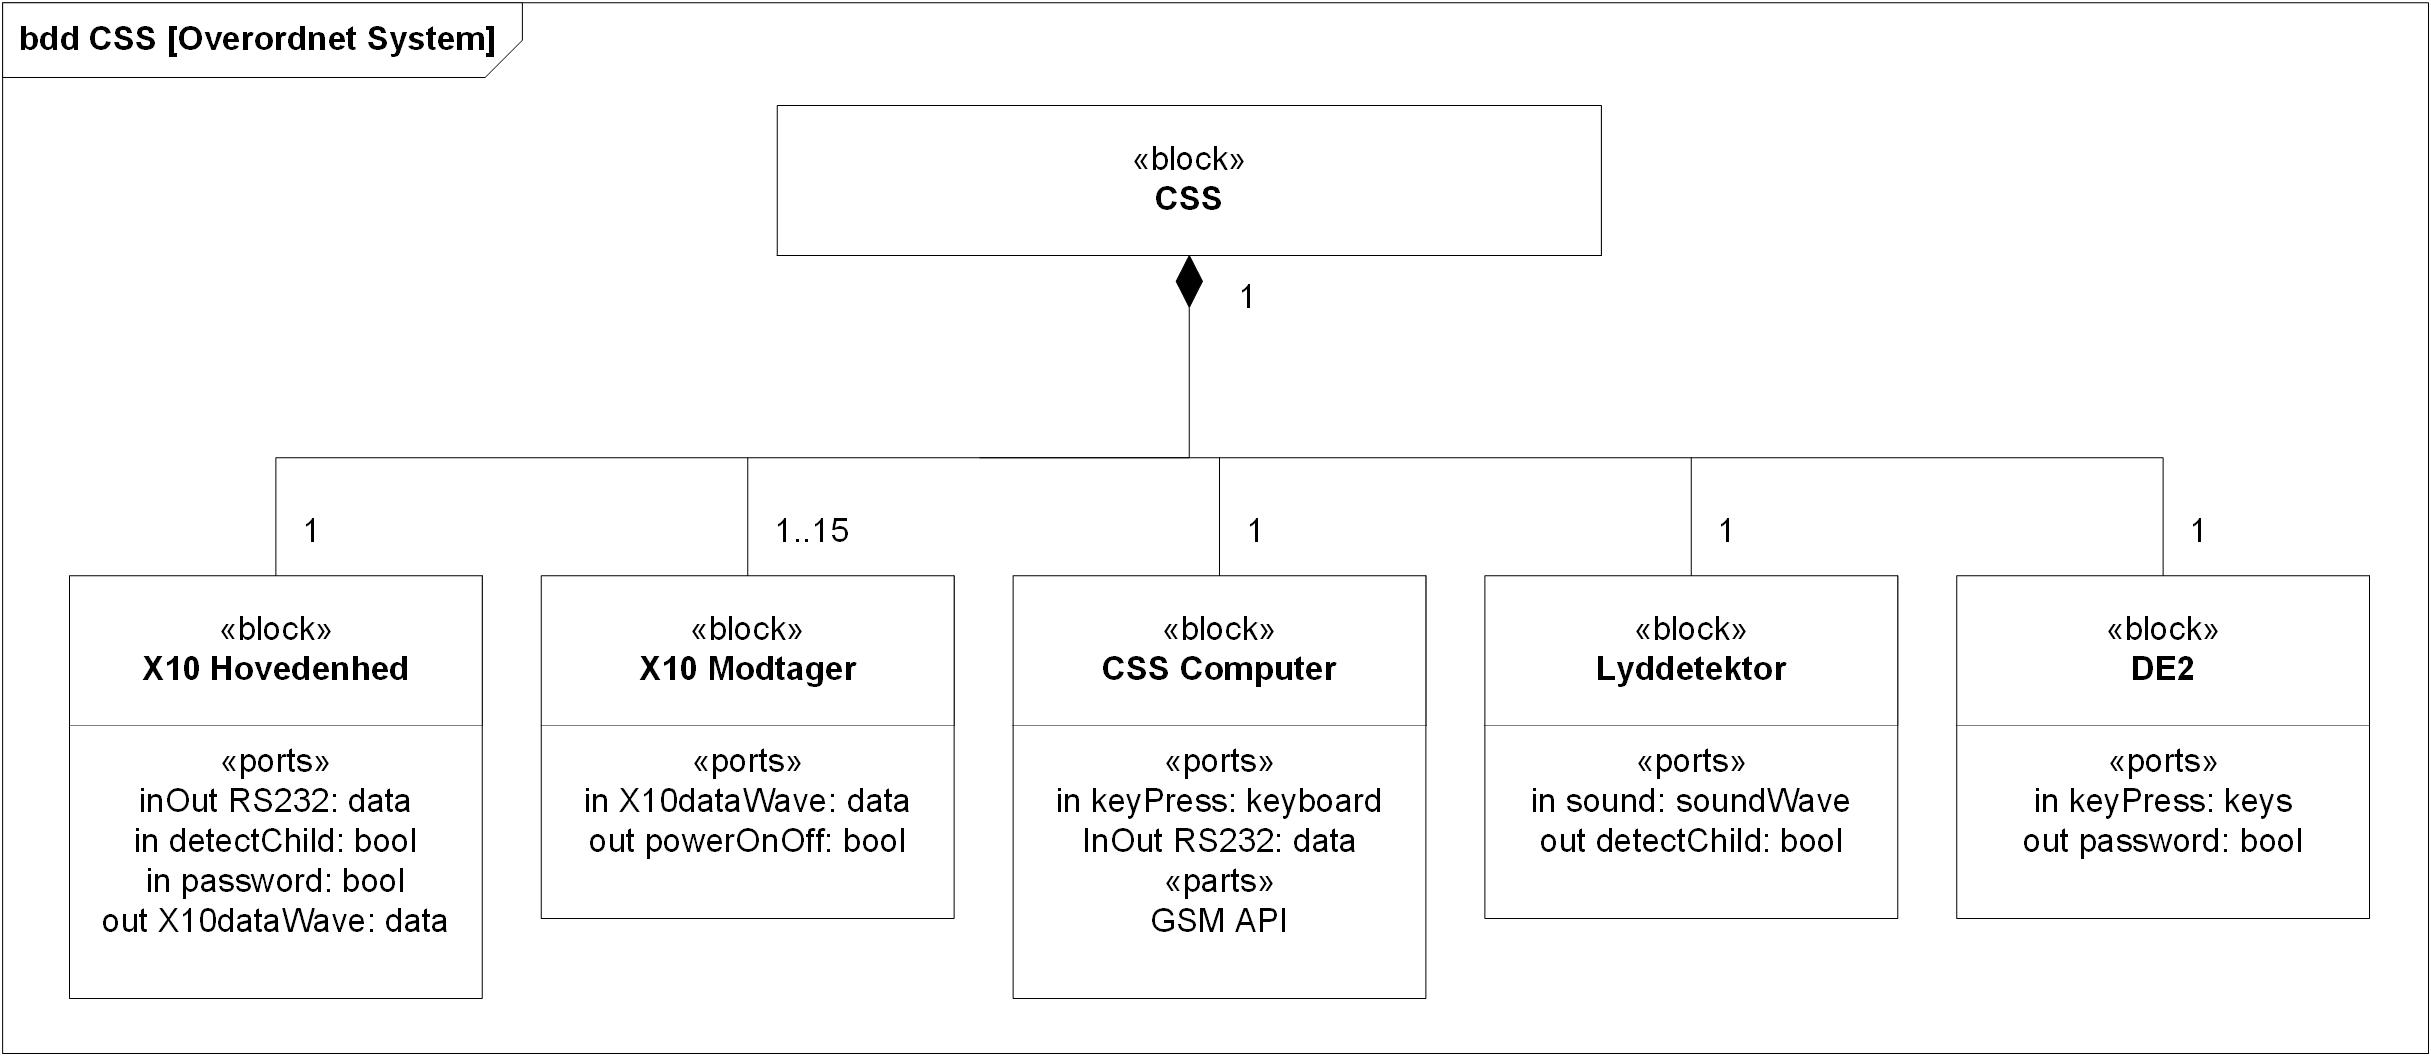
\includegraphics[width=0.9\textwidth]{billeder/diagrammer/BDD_Hardware}}
\caption{BDD Hardware}
\label{lab:bddhardware}
\end{figure}

\begin{figure}[!htbp] \centering
\subsection{BDD Hovedenhed}
{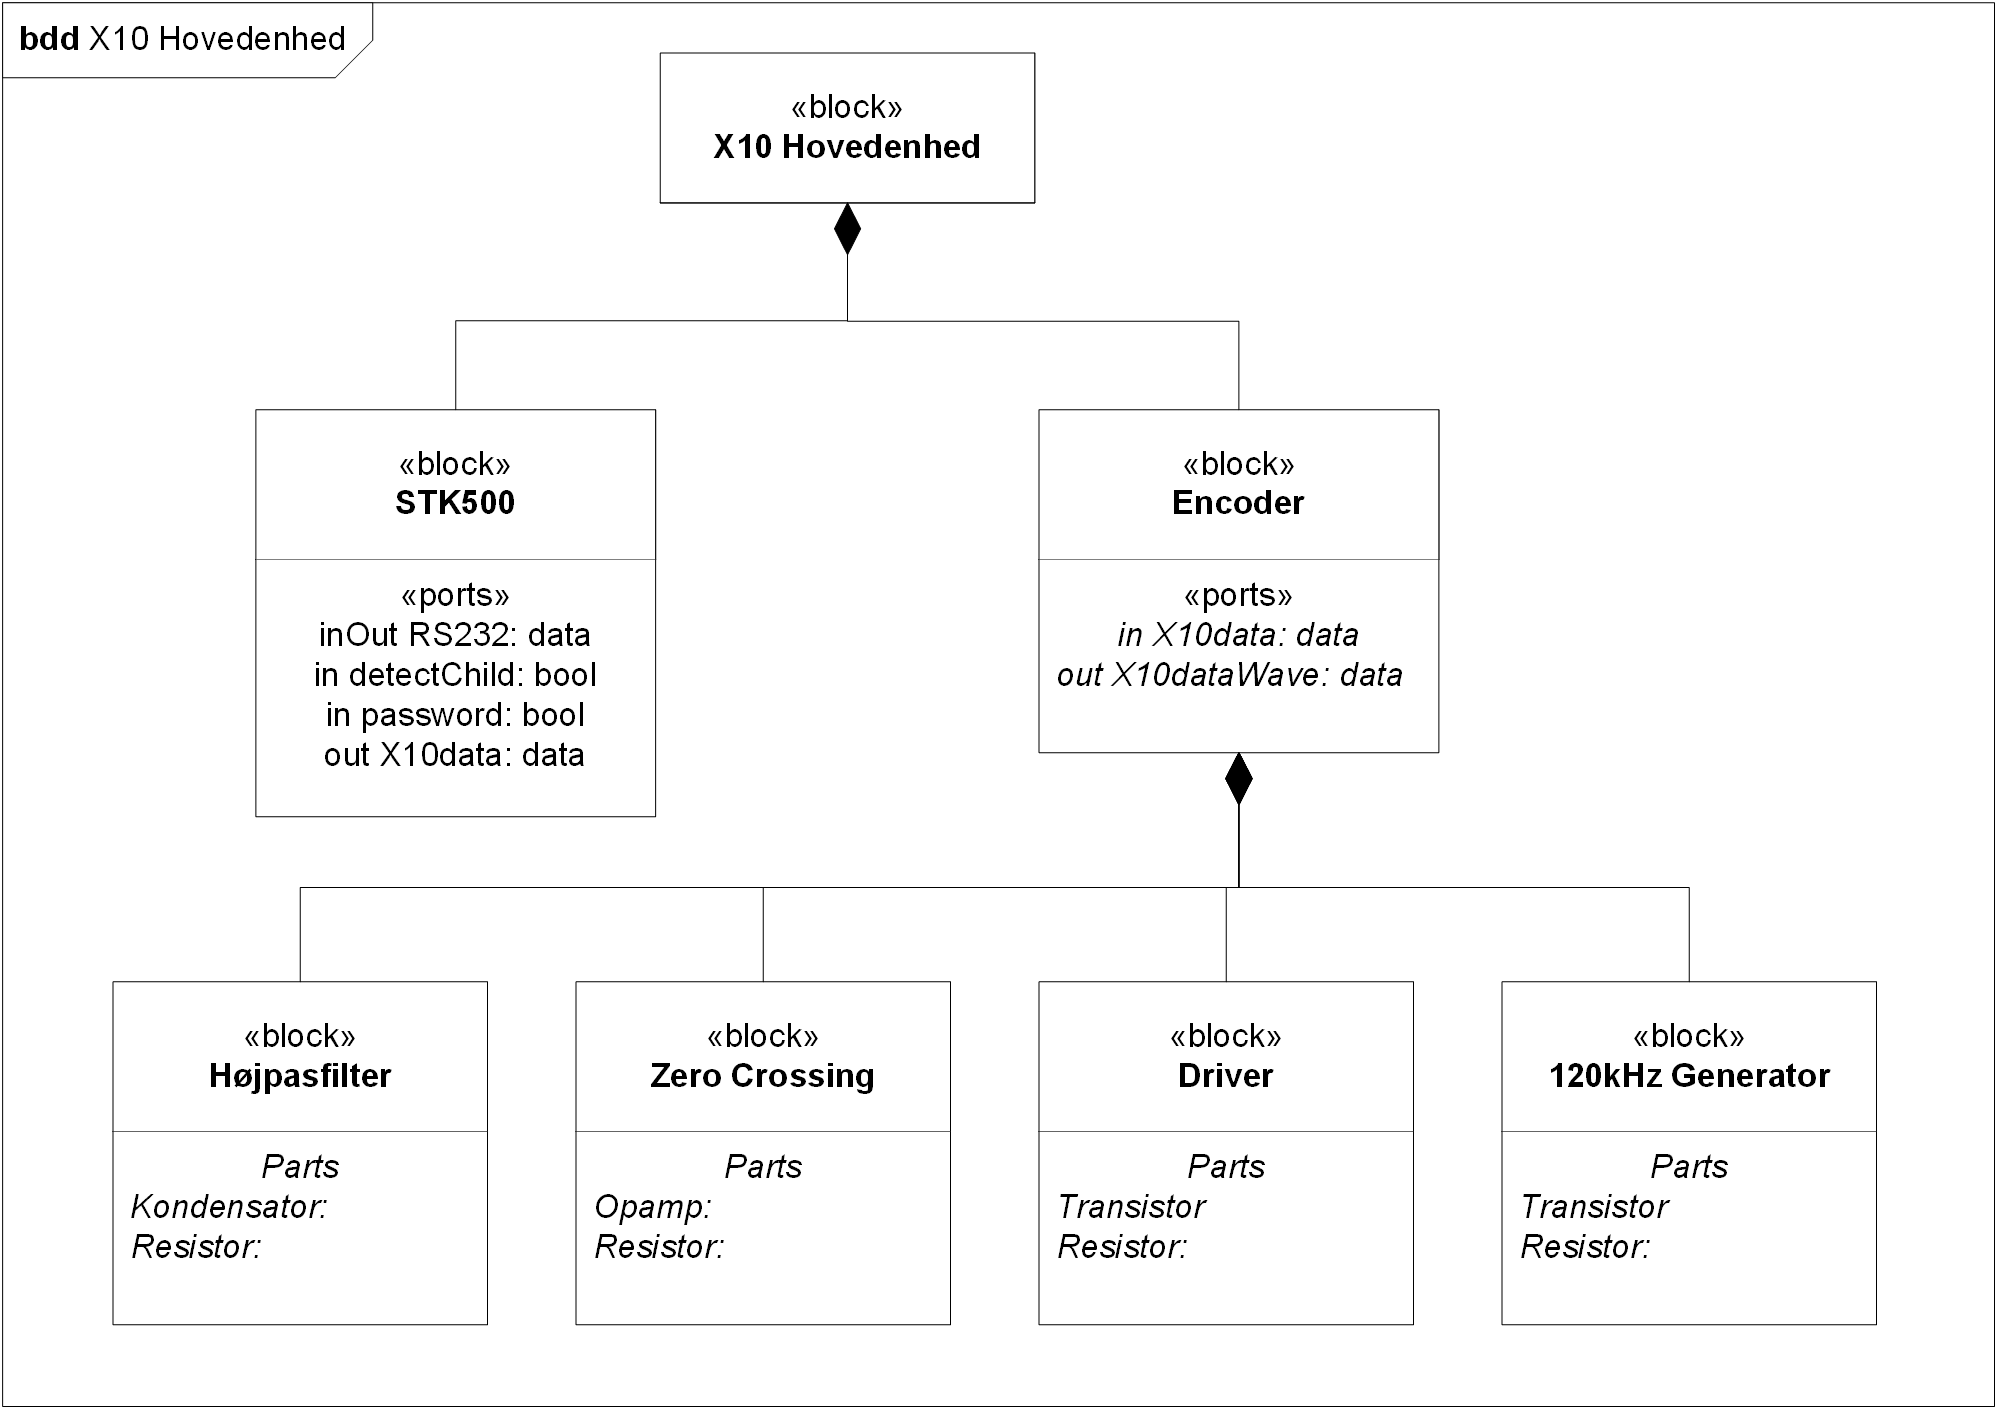
\includegraphics[width=0.9\textwidth]{billeder/diagrammer/BDD_Hovedenhed}}
\caption{BDD Hovedenhed}
\label{lab:bddhovedenhed}
\end{figure}

\begin{figure}[!htbp] \centering
\subsection{BDD Modtager}
{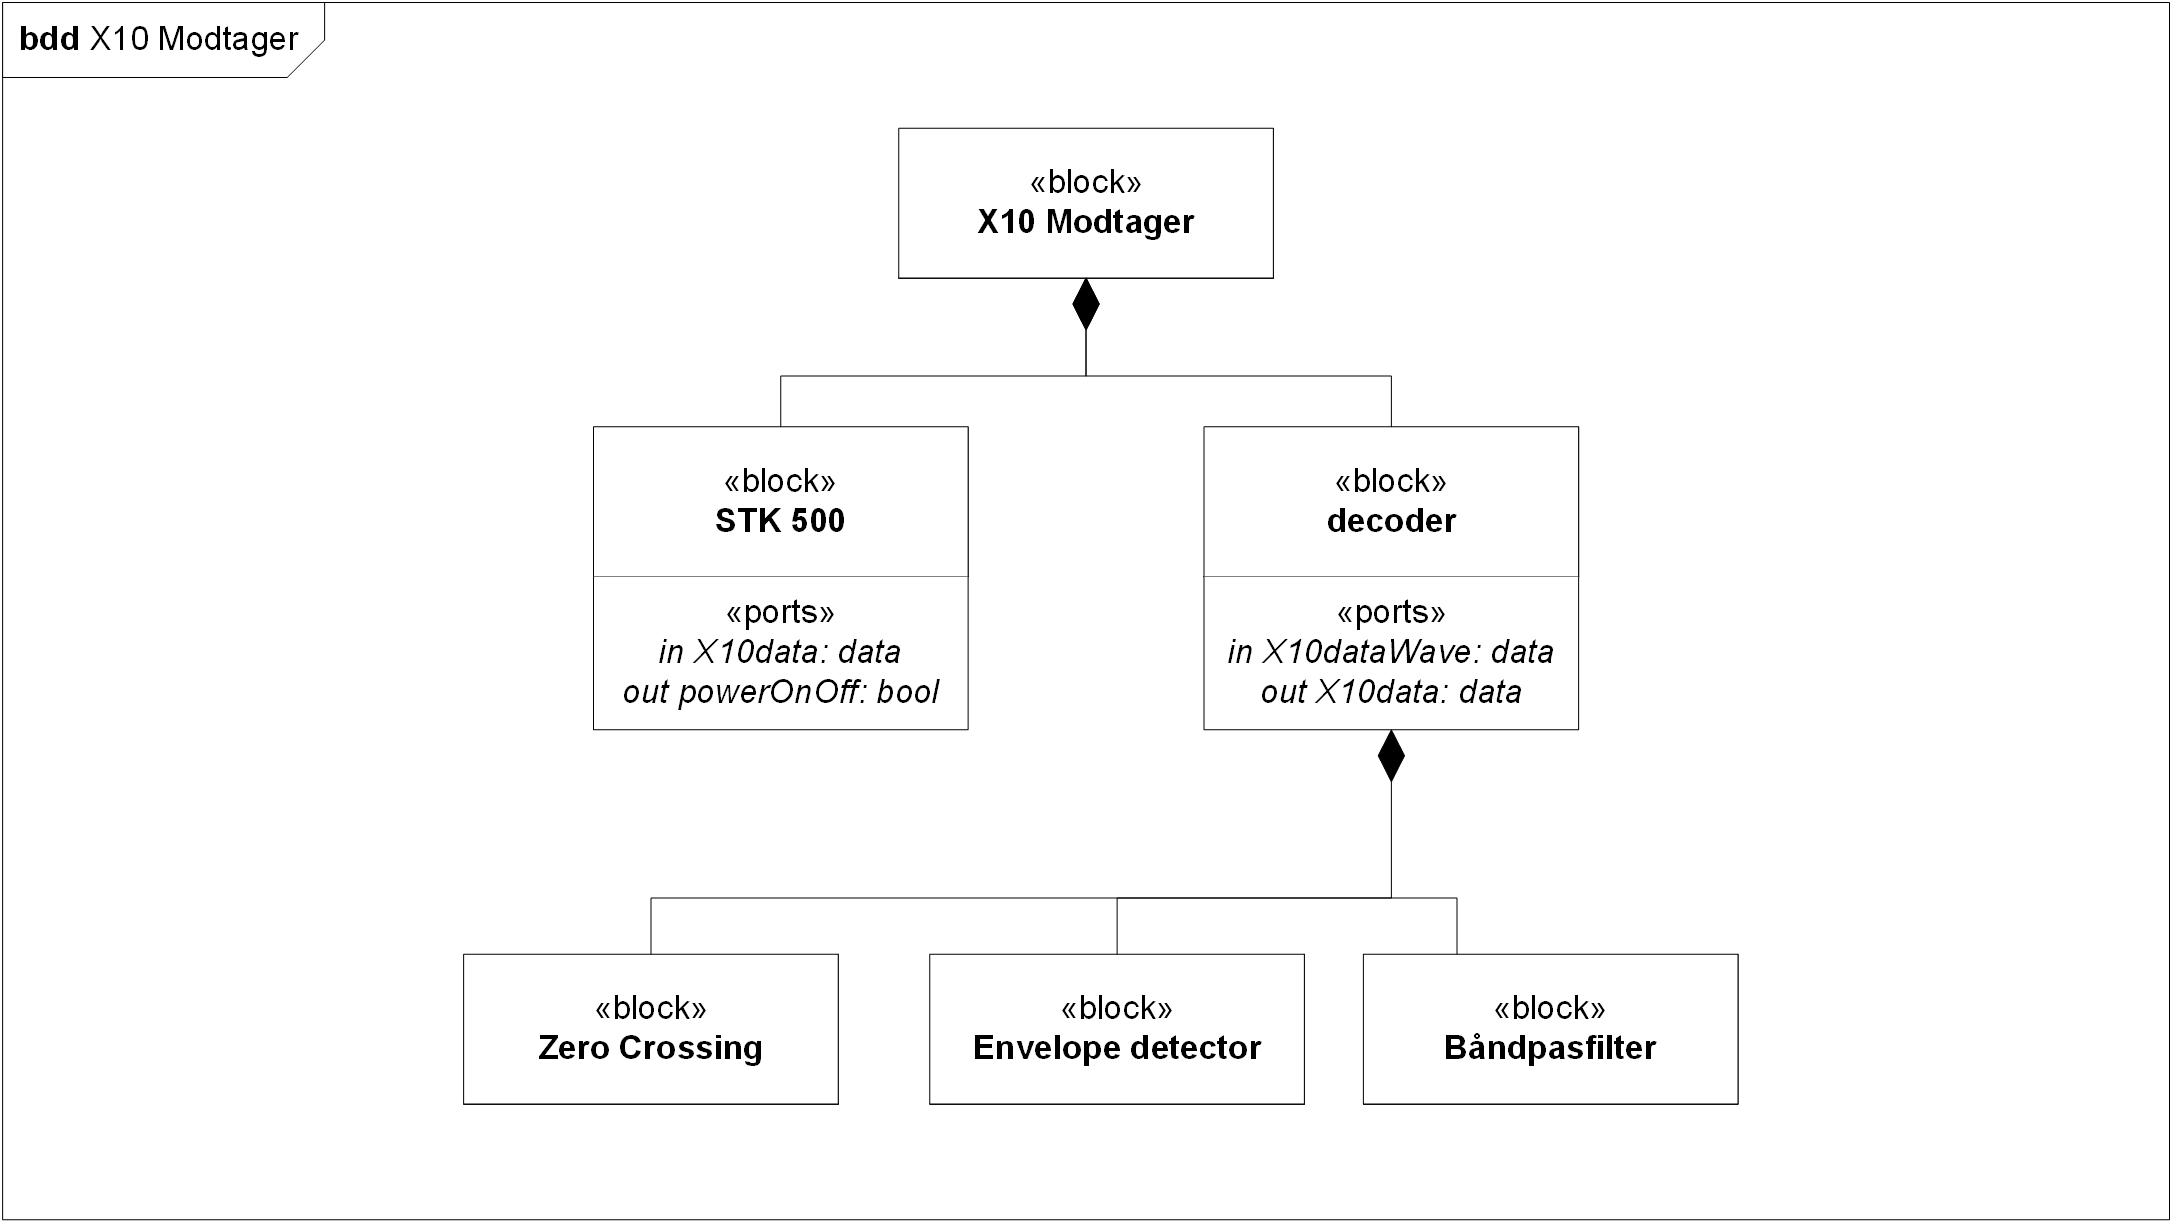
\includegraphics[width=0.9\textwidth]{billeder/diagrammer/BDD_Modtager}}
\caption{BDD Modtager}
\label{lab:bddmodtager}
\end{figure}

\begin{figure}[!htbp] \centering
\subsection{IBD Hardware}
{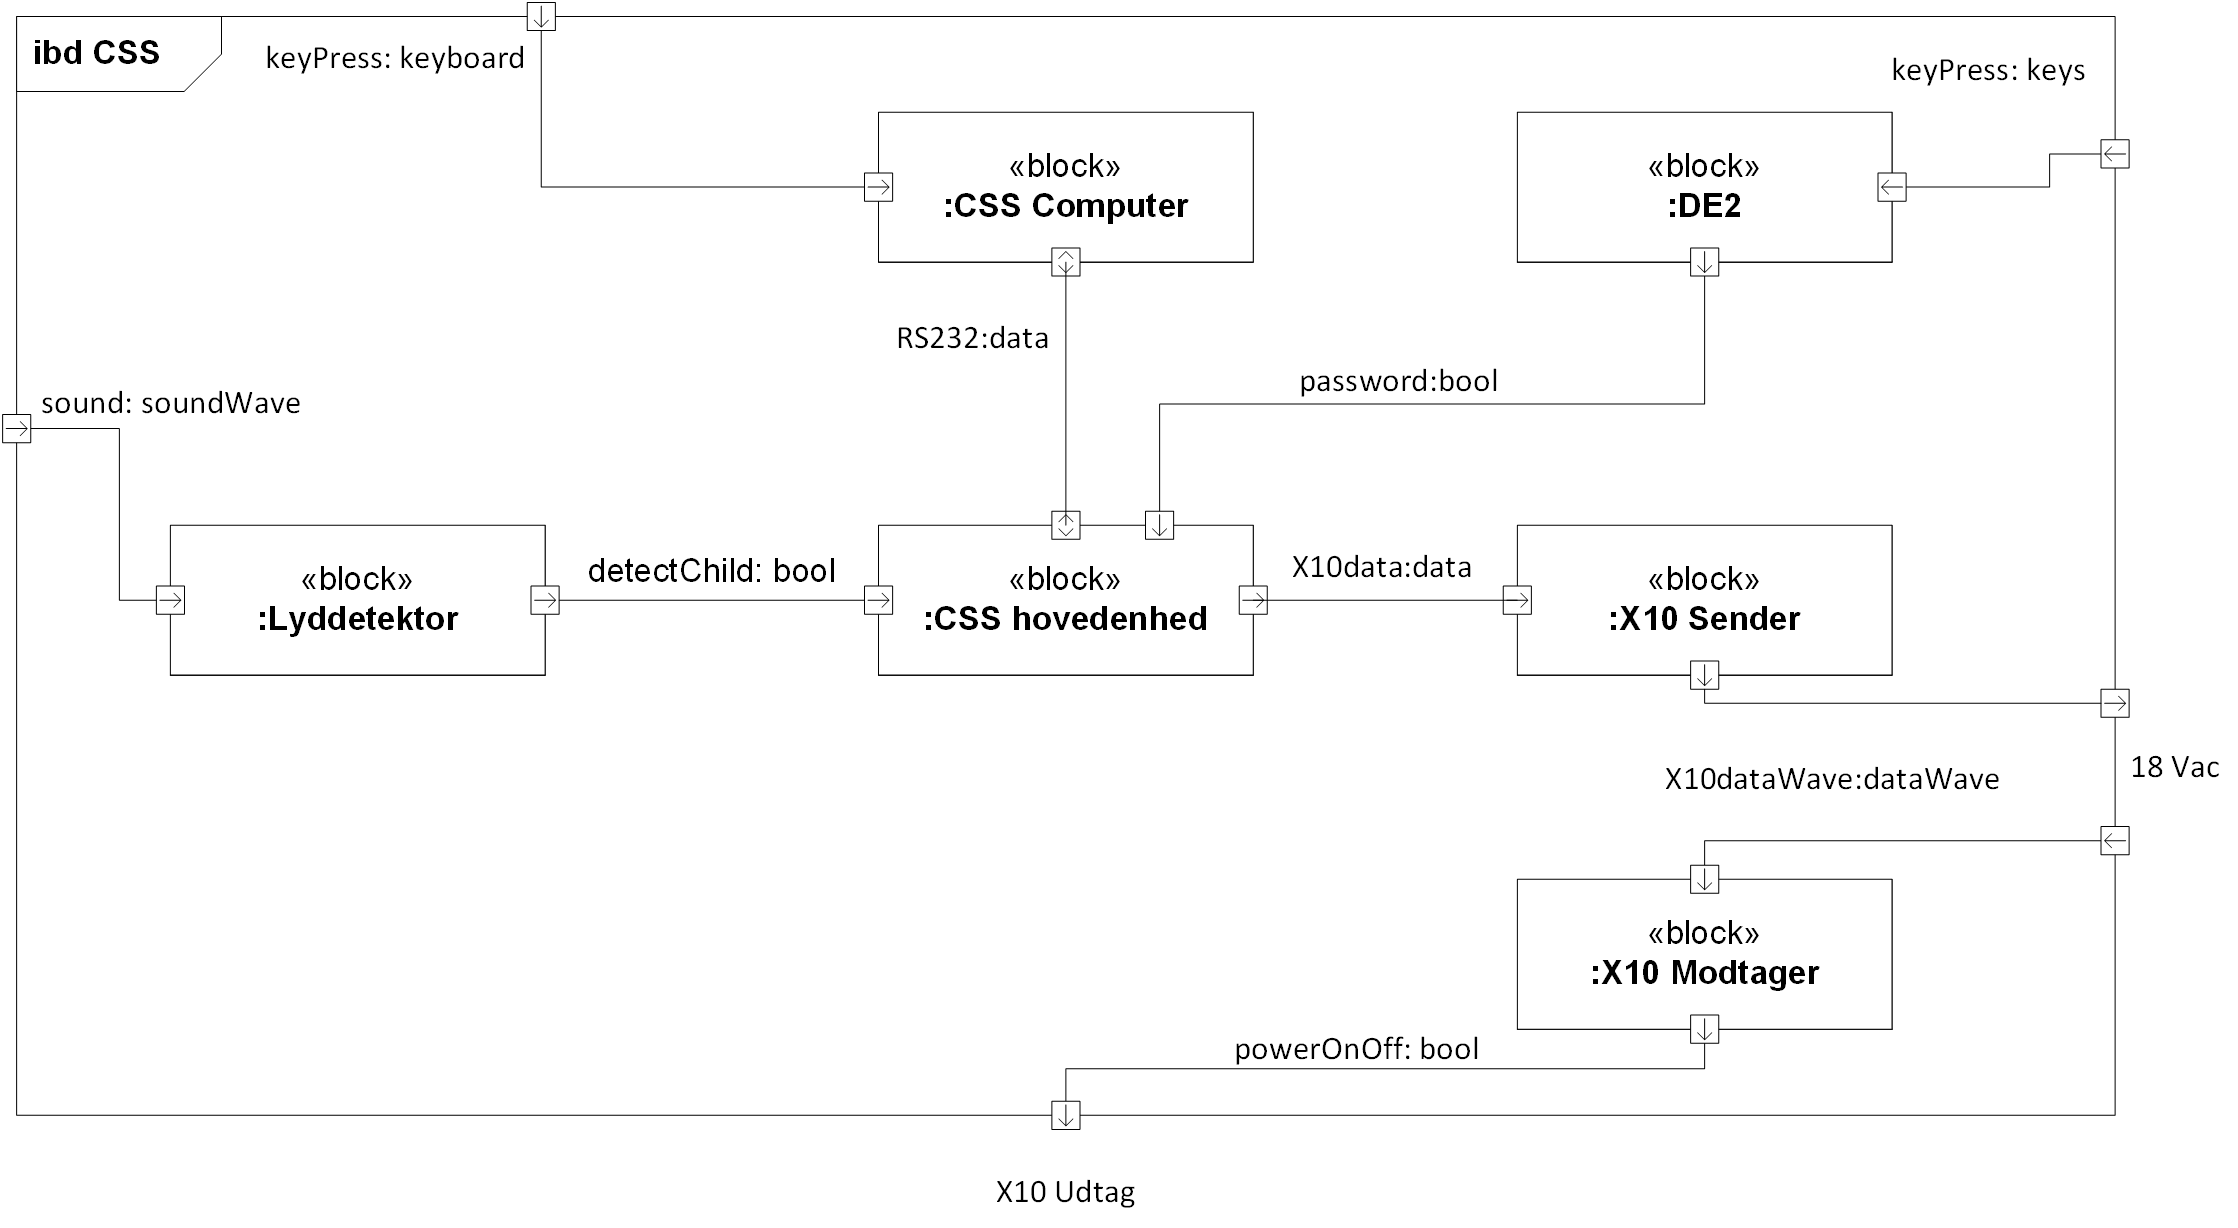
\includegraphics[width=0.9\textwidth]{billeder/diagrammer/IBD_Hardware}}
\caption{IBD Hardware}
\label{lab:ibdhardware}
\end{figure}

\begin{figure}[!htbp] \centering
\subsection{IBD Hovedenhed og Modtager}
{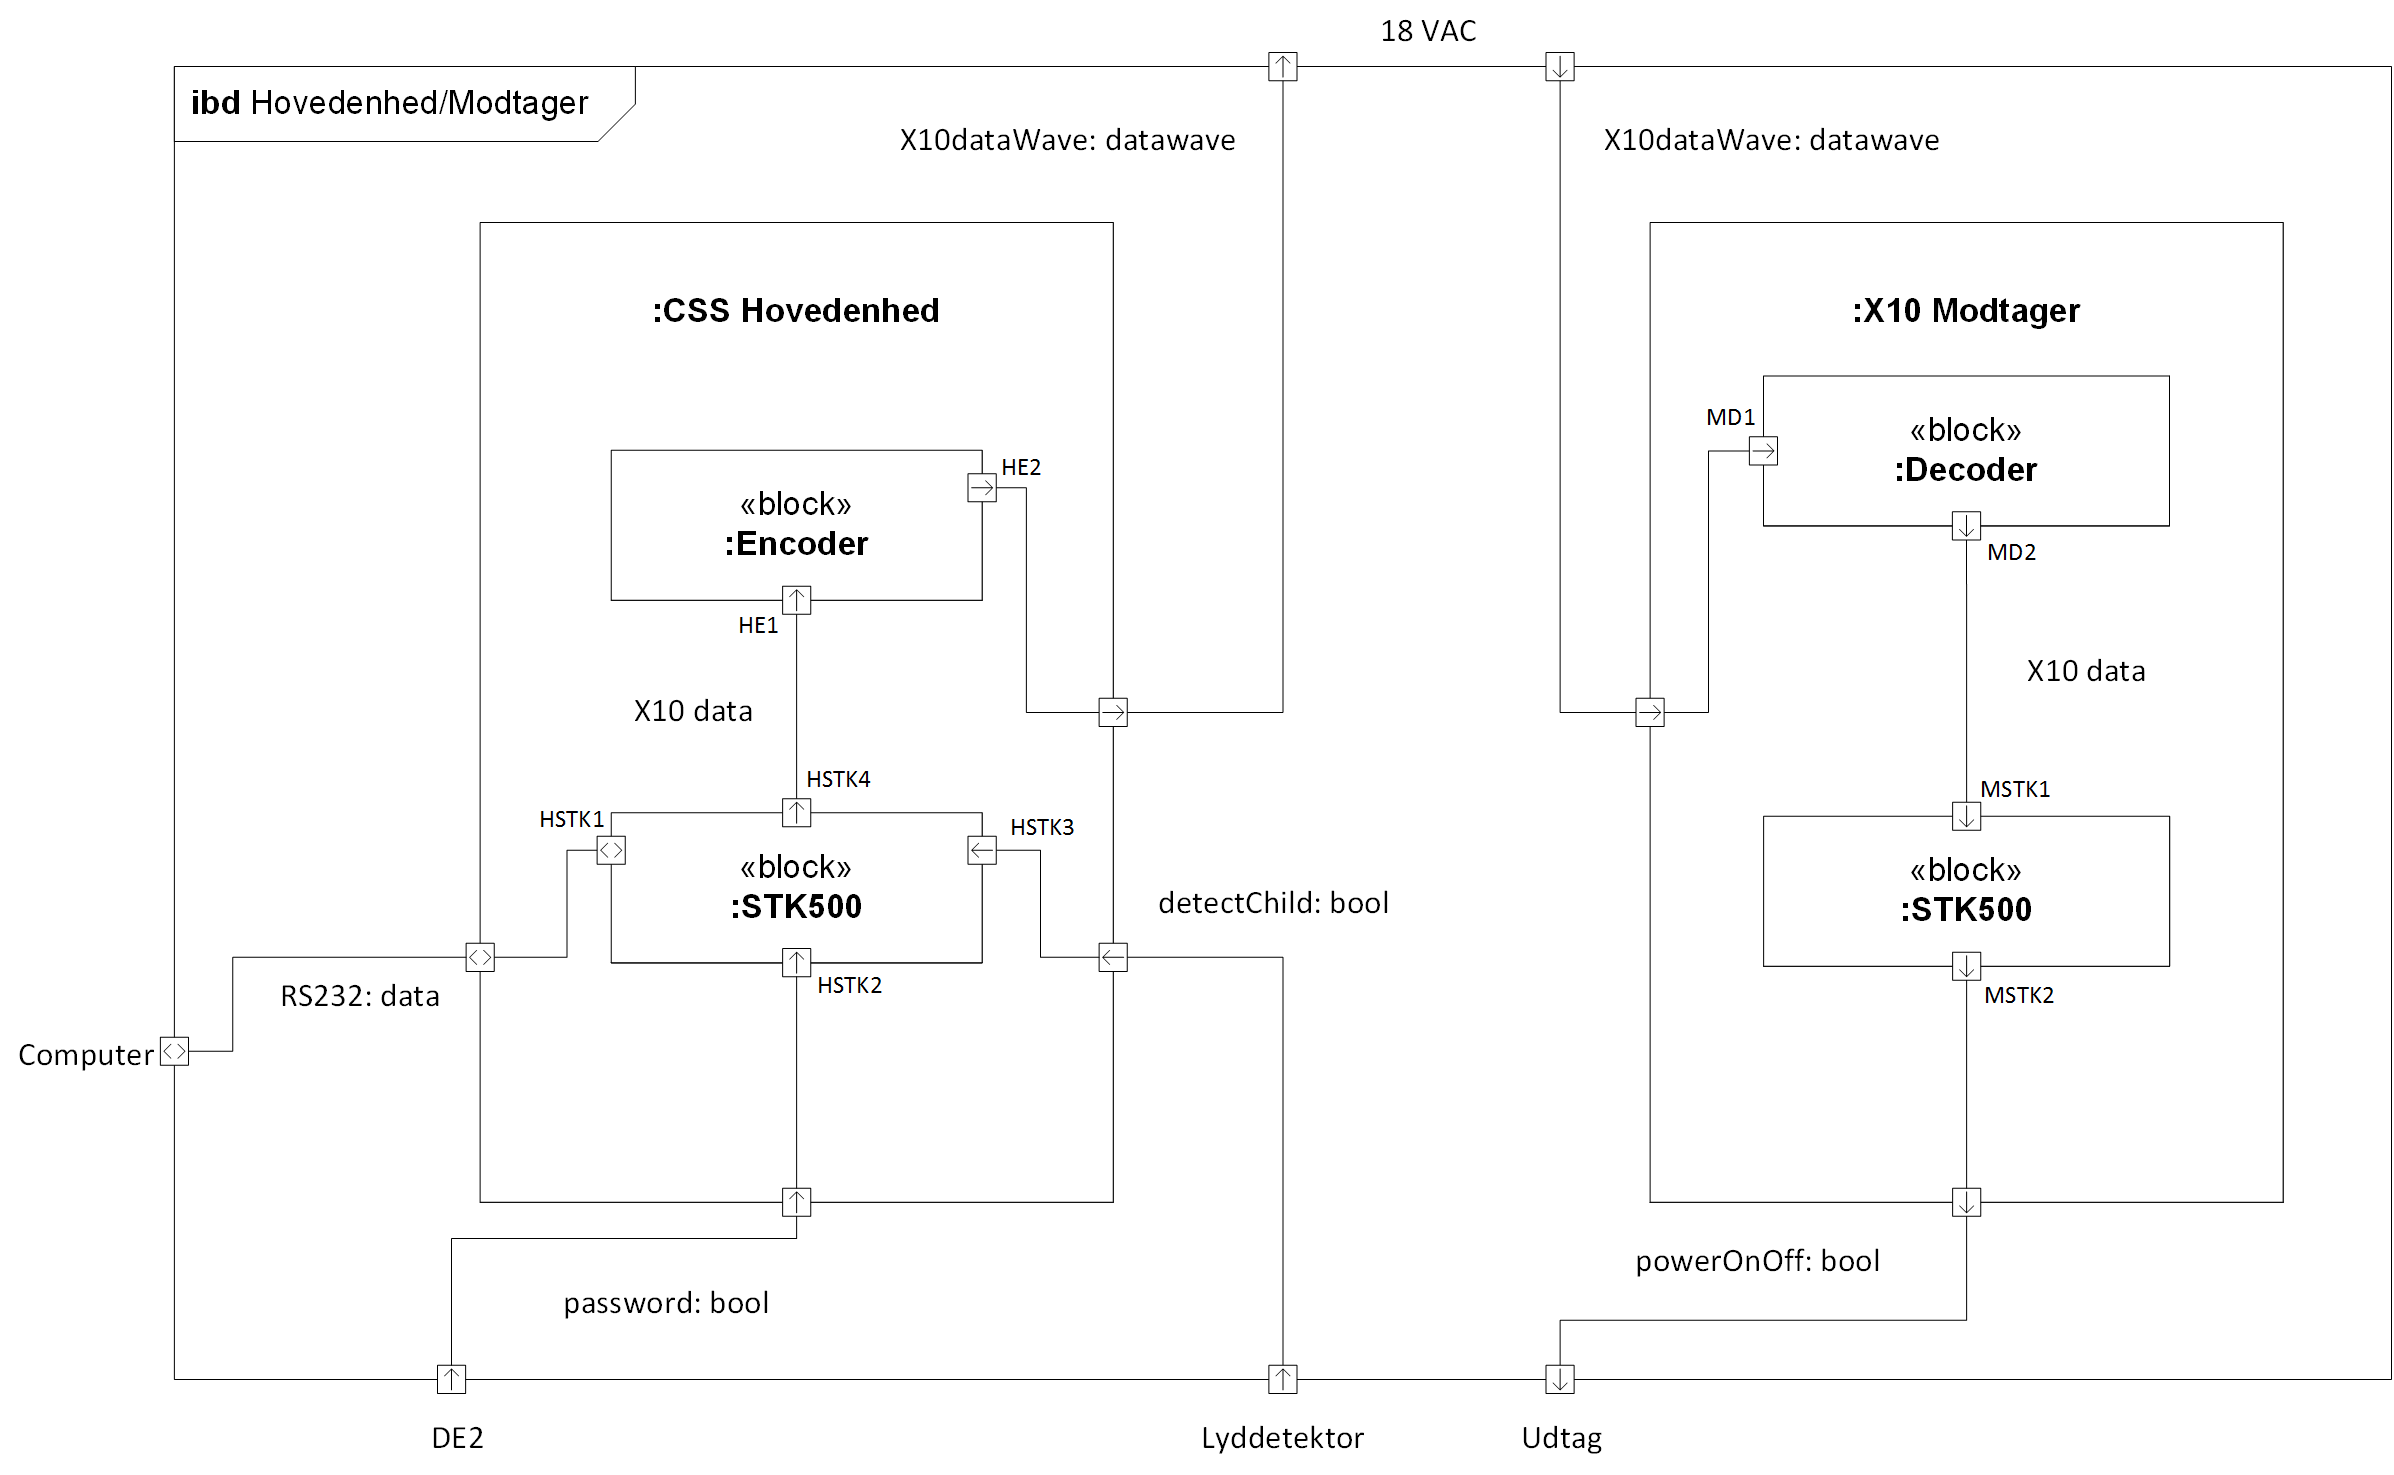
\includegraphics[width=0.9\textwidth]{billeder/diagrammer/IBD_Hovedenhed_Modtager}}
\caption{IBD Hovedenhed og Modtager}
\label{lab:ibdhovedenhedmodtager}
\end{figure}

\clearpage
\newpage

\begin{table}[htbp] %% Blok og Signal Tabel
\subsection{Grænseflade}
For at opnå forståelse for signaler mellem blokkene laves en grænseflade der beskriver de enkelte blokkes porte og hvilke signaler der løber mellem disse.

\subsubsection{Blok beskrivelse}
Til at beskrive blokkene nærmere er anvendt tabeller som ses herunder. Her er hvert signal i en respektiv blok kommenteret og blokkens funktion er kort beskrevet. 

\begin{tabular}{|p{3,3cm}|p{3,3cm}|p{3,3cm}|p{3,3cm}|}
\hline
\textbf{Bloknavn} & \textbf{Funktion} & \textbf{Signaler} & \textbf{Kommentar} \\ \hline

Encoder & modtage kommando og encode til 120 kHz bursts & 120 kHz & Data ud \\ \cline{3-4}	
& & X10 data & X10 data kommando ind \\ \hline

STK500 Hovedenhed & Genererer burst og detekterer på zero-crossing & RS232 & Laptop forbindelse \\ \cline{3-4}
& & X10 data & X10 data kommando linje \\ \cline{3-4}
& & Bool & lyd detektion \\ \cline{3-4}
& & Bool & Password accept \\ \hline

Decoder & Modtager 120 kHz og decoder til X10 data & 120 kHz & 120 kHz ind \\ \cline{3-4}
& & X10 data & Kommando linje \\ \cline{3-4}
& & 120 kHz & 120 kHz data ind \\ \hline

STK 500 Decoder & Modtager burst og detekterer på zero-crossing & X10 data & X10 data ind \\ \cline{3-4}
&& Bool & Power I/O ekstern enhed \\ \hline 
\end{tabular}

\subsubsection{Signal beskrivelse}
For at fuldende beskrivelsen af grænsefladen er der lavet en signaltabel som kan ses herunder. Hvert signal er beskrevet og tilknyttet en kort kommentar. Området et signal er defineret under er også beskrevet. Blok og terminal indgår også. 

\begin{tabular}{|p{2cm}|p{2cm}|p{2cm}|p{2cm}|p{2cm}|p{2,2cm}|}
\hline
\textbf{Signal-navn} & \textbf{Funktion} & \textbf{Område} & \textbf{Port 1} & \textbf{Port 2} & \textbf{Kommentar} \\ \hline

120 kHz & sende kommando på 18V nettet & & Encoder, HE2 & Decoder, DM1 & \\ \hline

X10 data & kommando & & STK500, HSTK4 & Encoder, HE1 & \\
&&& Decoder, MD2 & STK500, MSTK500 &\\ \hline

\end{tabular} 
\end{table}